\chapter{Risultati}
\label{cap:risultati}

\textit{\indent Questo capitolo presenta un'analisi dettagliata dei risultati ottenuti dagli esperimenti descritti nel capitolo precedente e una riflessione su di essi.}

\section{Risultati degli Esperimenti QUIC}
\subsection{Risultati Esperimento 1}
\begin{figure}[h!]
    \centering
    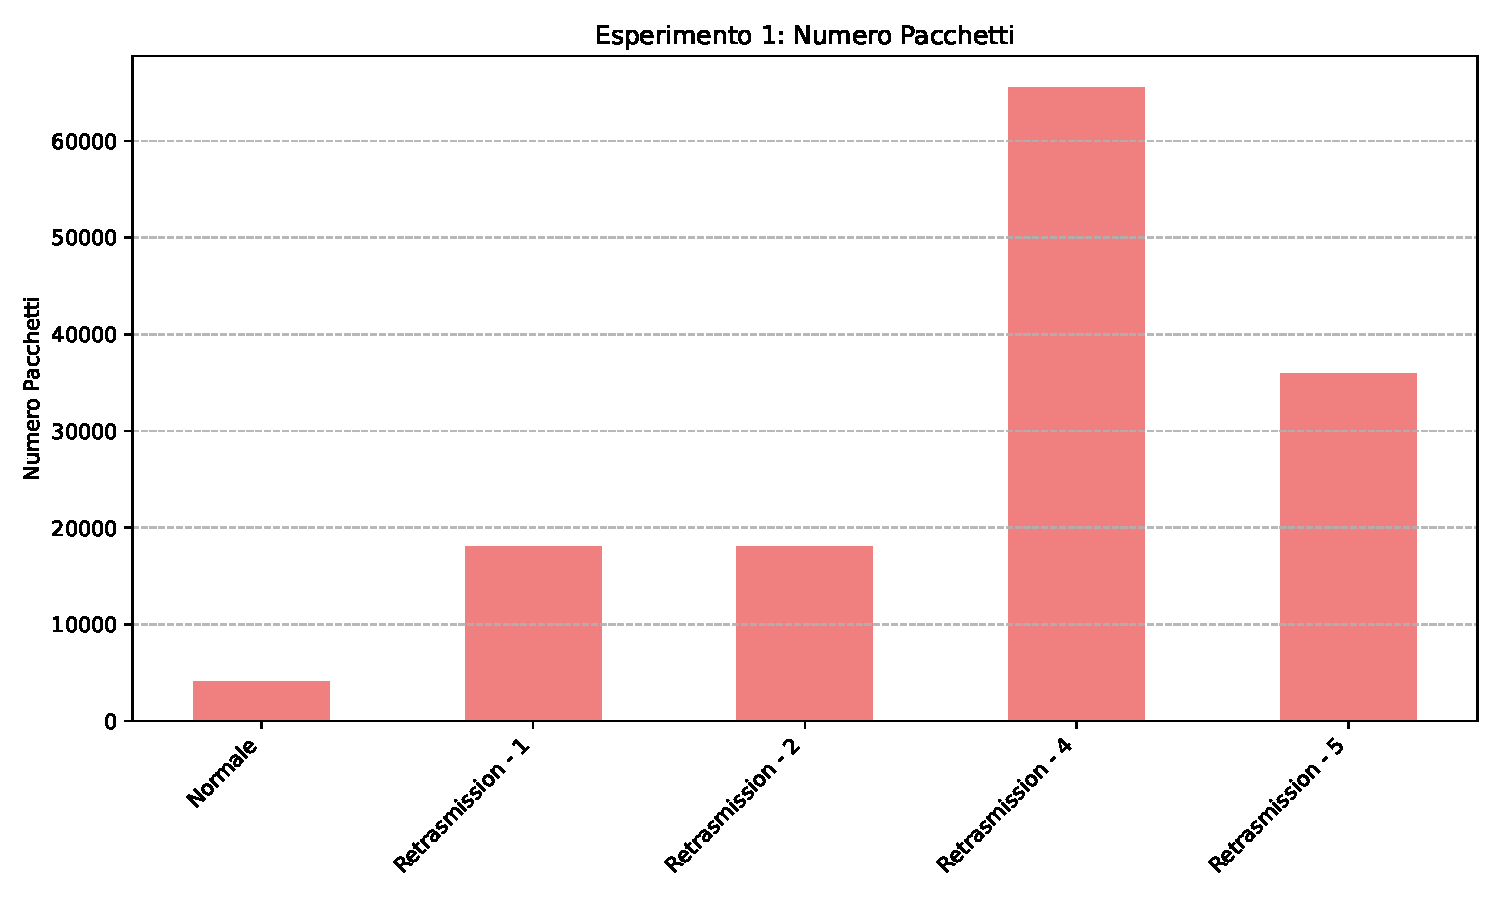
\includegraphics[width=\textwidth]{graphNumPacchetti1.pdf}
    \caption{Descrizione del grafico}
    \label{fig:grafico1}
\end{figure}
\begin{figure}[h!]
    \centering
    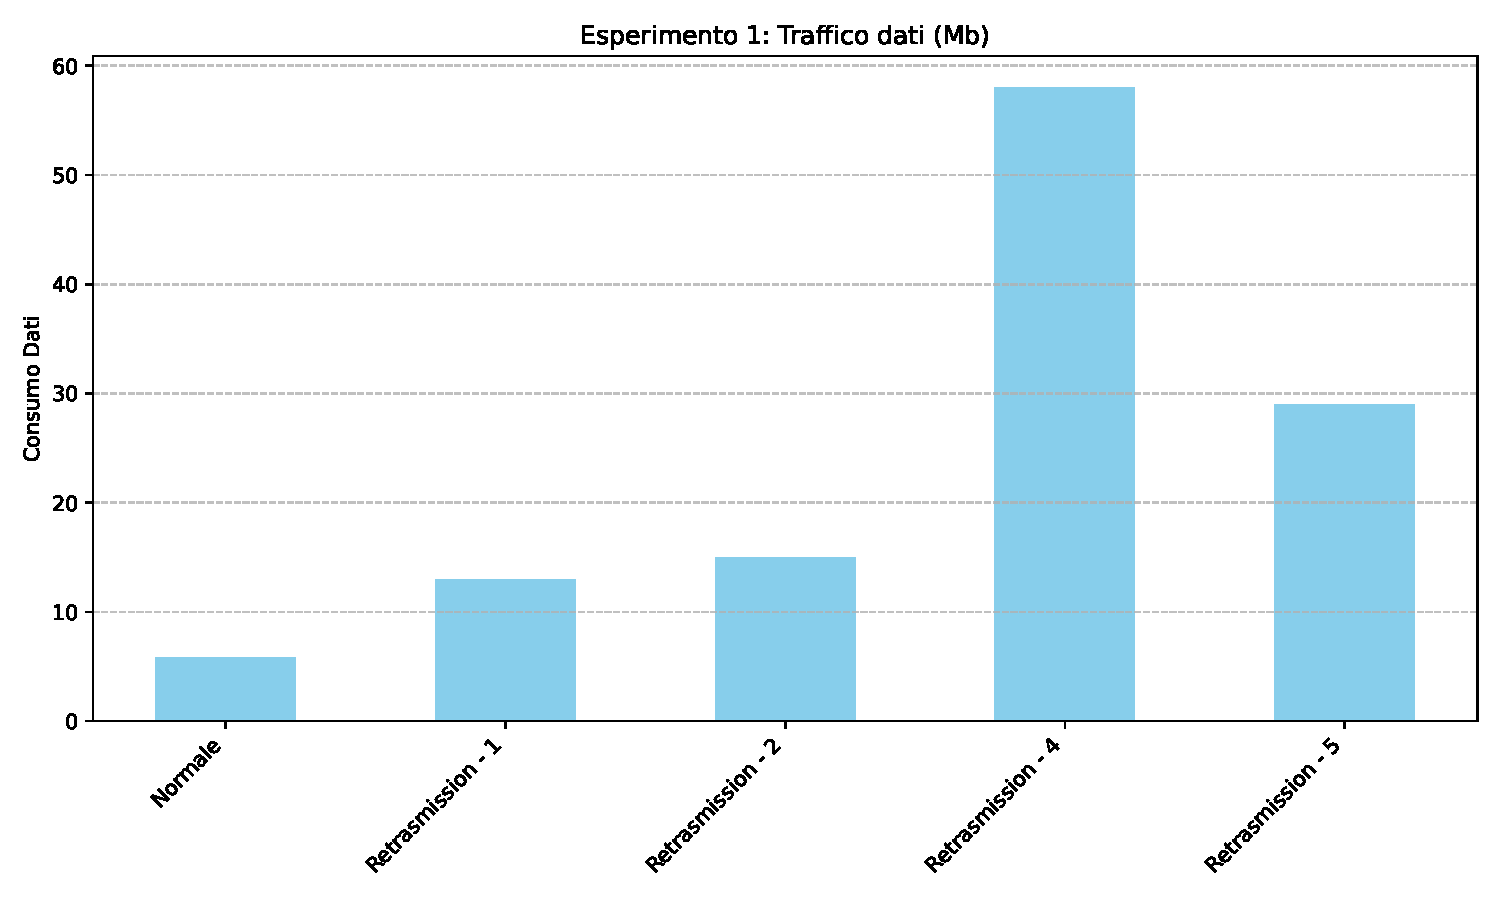
\includegraphics[width=\textwidth]{graphTraffico1.pdf}
    \caption{Descrizione del grafico}
    \label{fig:grafico12}
\end{figure}
\subsection{Risultati Esperimento 2}
\begin{figure}[h!]
    \centering
    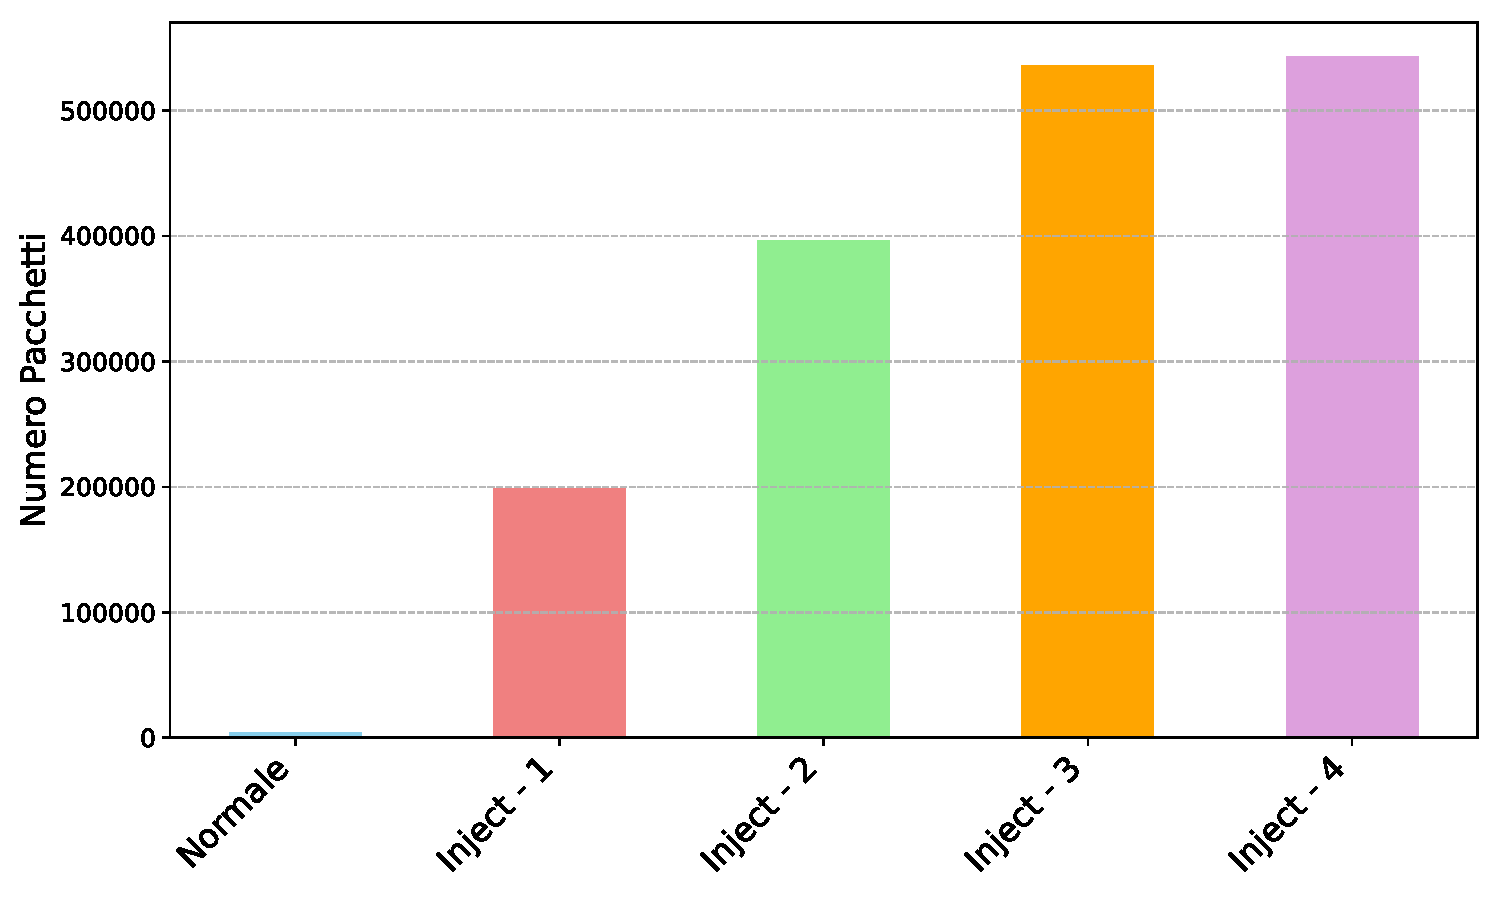
\includegraphics[width=\textwidth]{graphNumPacchetti2.pdf}
    \caption{Descrizione del grafico}
    \label{fig:grafico2}
\end{figure}
\begin{figure}[h!]
    \centering
    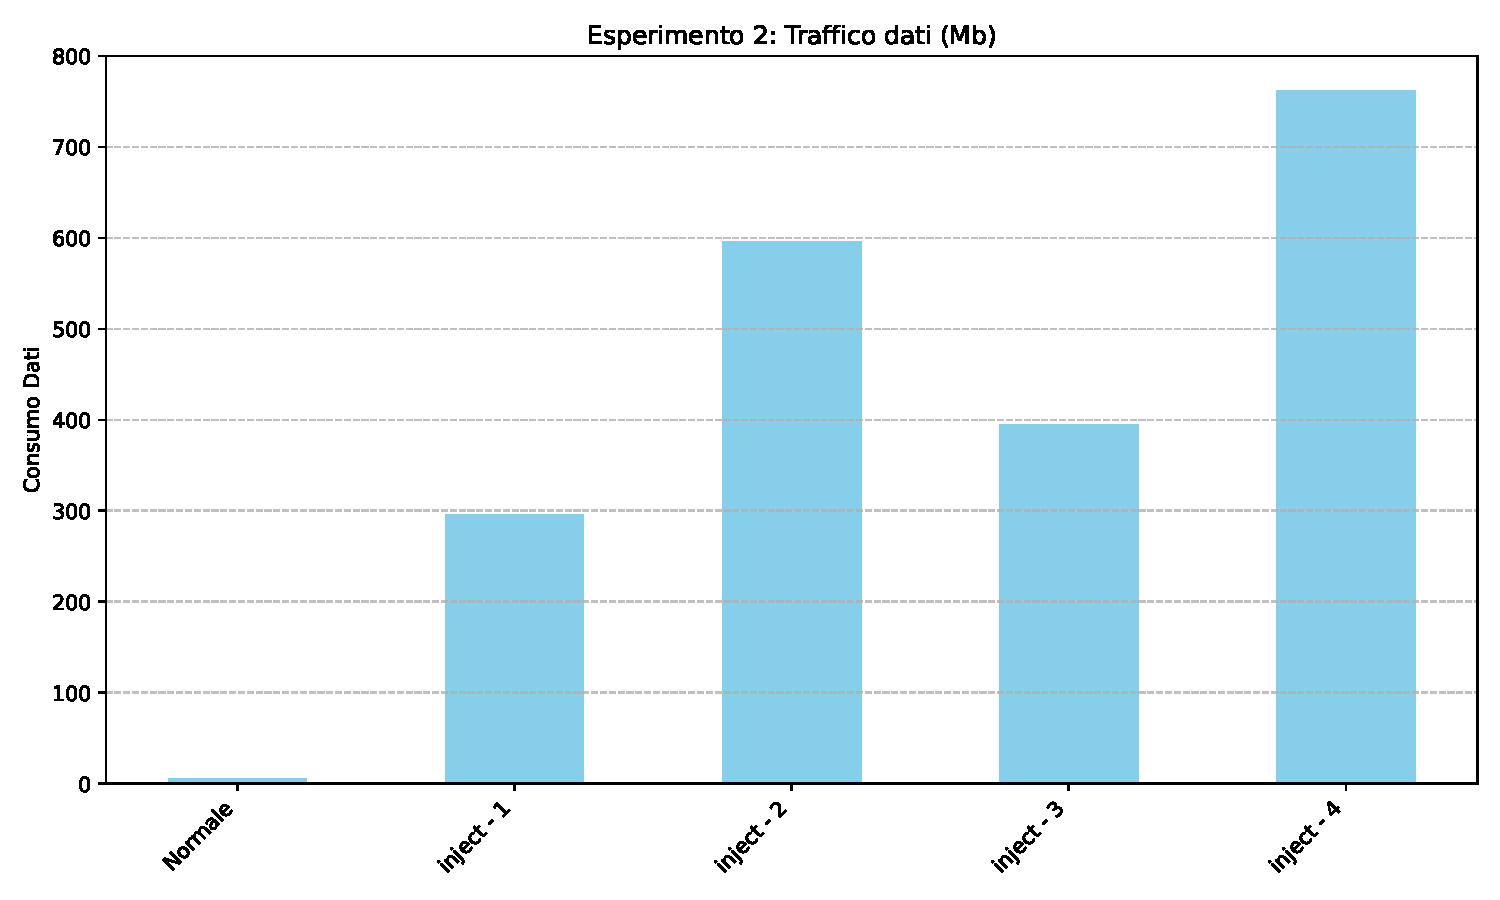
\includegraphics[width=\textwidth]{graphTraffico2.pdf}
    \caption{Descrizione del grafico}
    \label{fig:grafico12}
\end{figure}
\begin{figure}[h!]
    \centering
    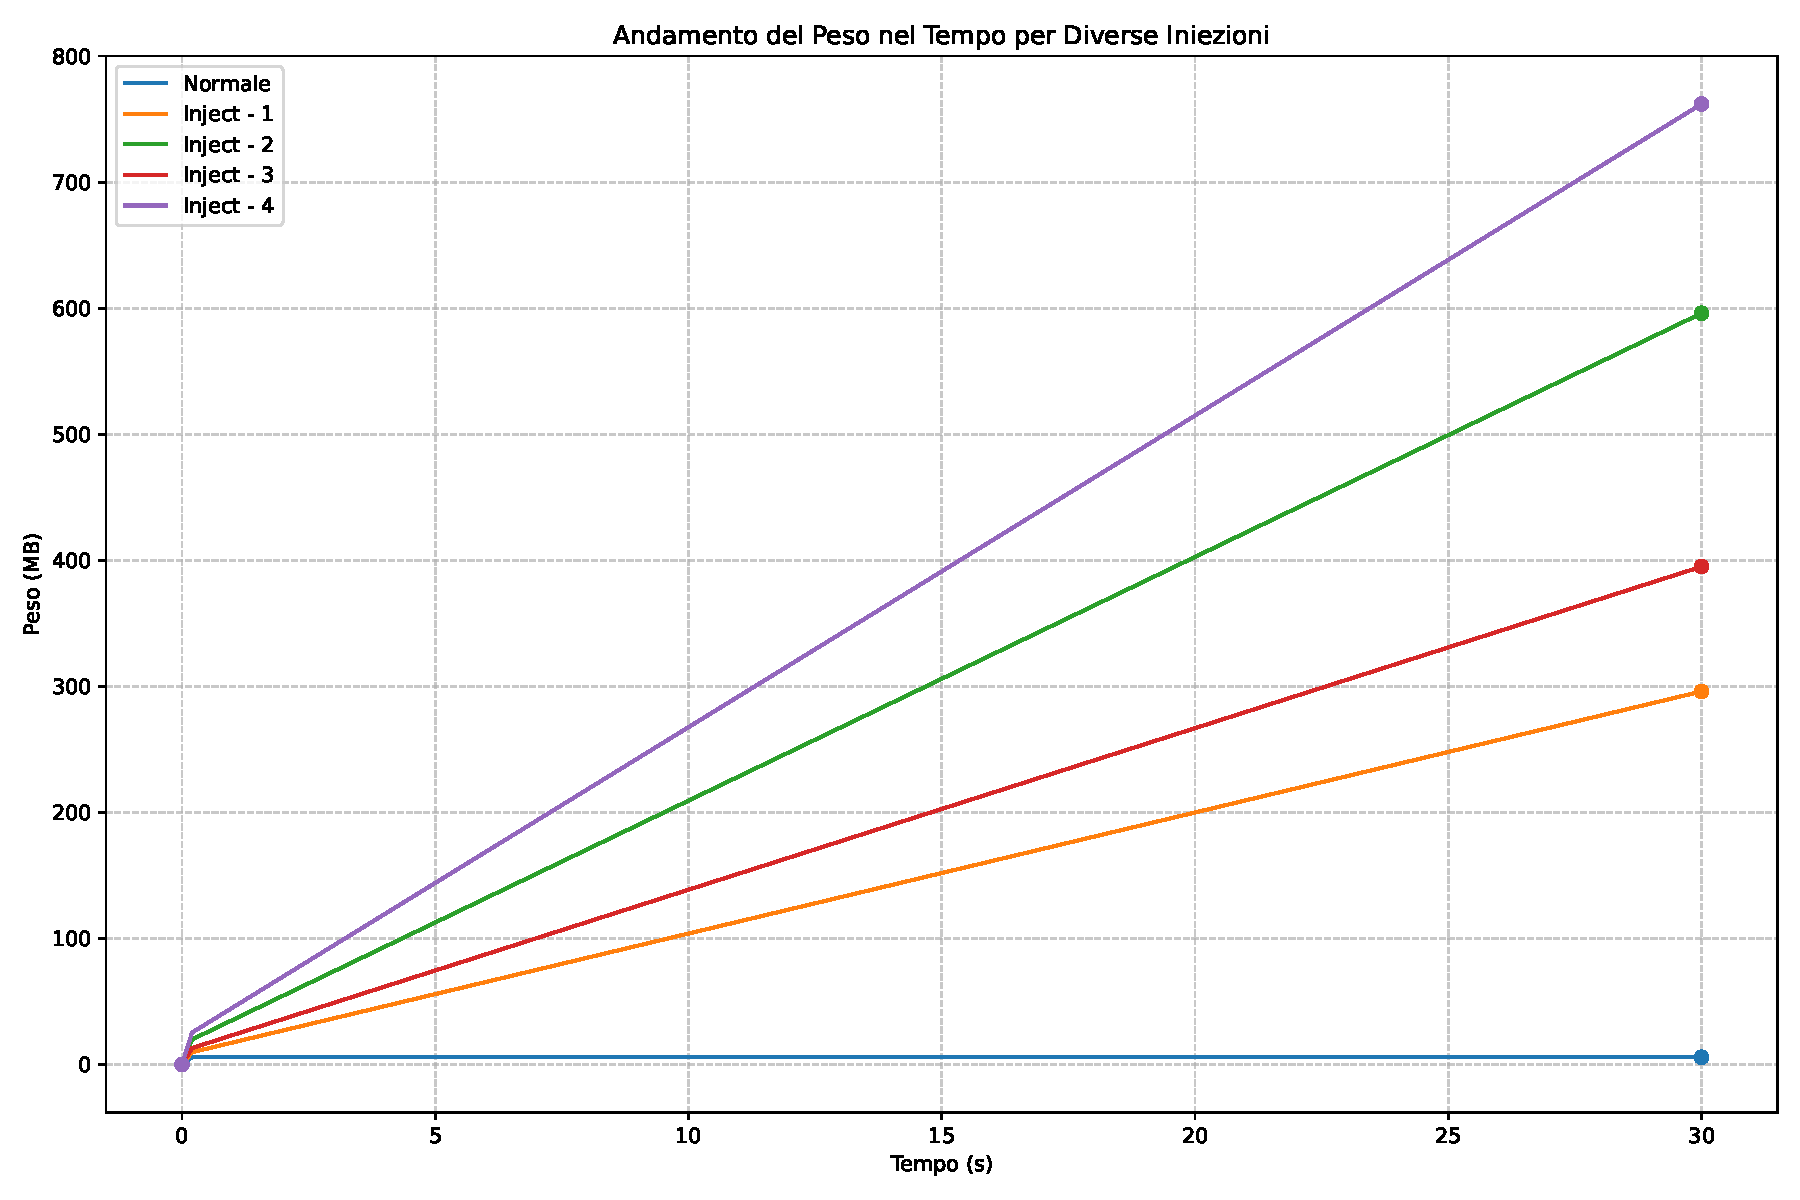
\includegraphics[width=\textwidth]{graphTrafficoTempo.pdf}
    \caption{Descrizione del grafico}
    \label{fig:grafico12}
\end{figure}
\subsection{Risultati Esperimento 3}
\begin{figure}[h!]
    \centering
    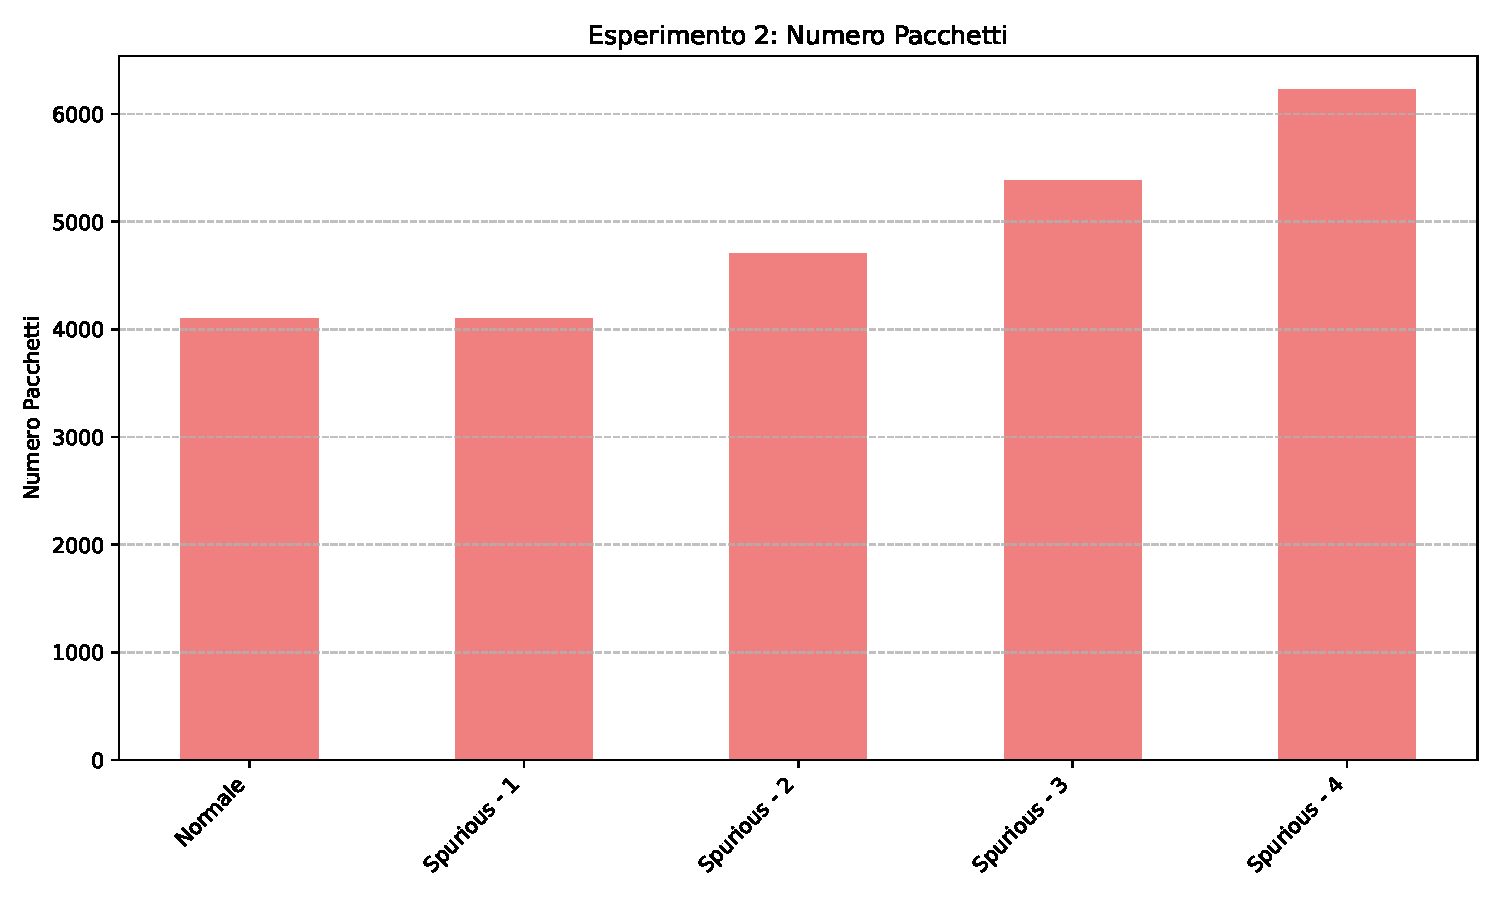
\includegraphics[width=\textwidth]{graphNumPacchetti3.pdf}
    \caption{Descrizione del grafico}
    \label{fig:grafico3}
\end{figure}
\begin{figure}[h!]
    \centering
    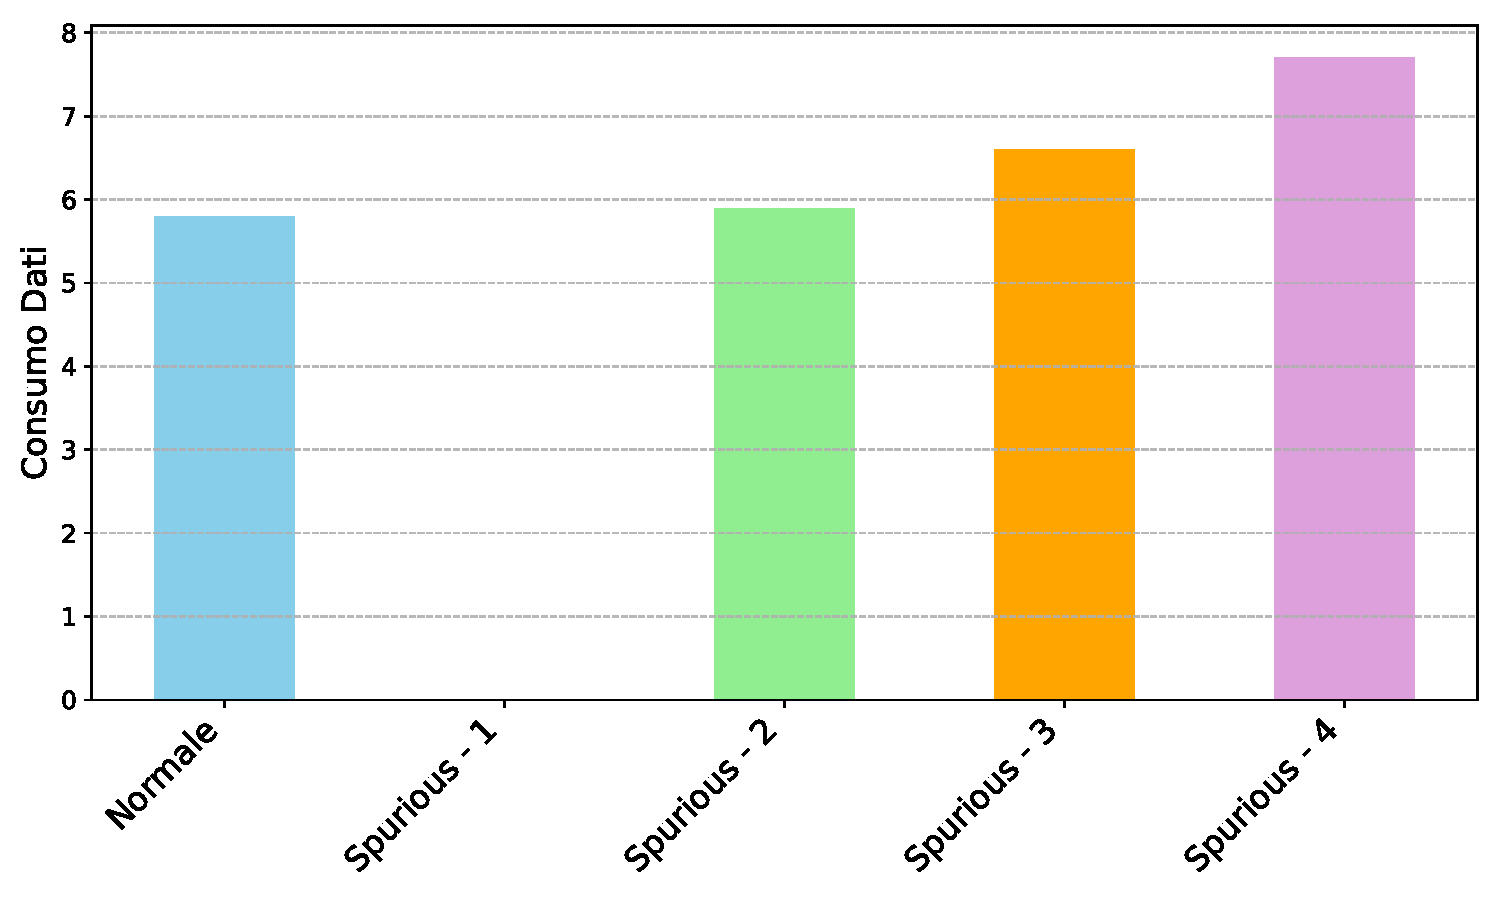
\includegraphics[width=\textwidth]{graphTraffico3.pdf}
    \caption{Descrizione del grafico}
    \label{fig:grafico12}
\end{figure}
